%% draft_sections_6.tex — NAACL 2027 SRW fragment (Section 6)
%% Restructured 2026-07: results lead with research findings (rating--sentiment,
%% AL scaling, human400 generalization), followed by provenance/evaluation
%% sensitivity and ablations. Labels sec:res-ablations / sec:res-human400 are
%% referenced from draft_4_5 and must be kept.
\section{Results and Analysis}
\label{sec:results}

\subsection{Rating--Sentiment Divergence Across Review Populations}
\label{sec:res-rating}

Star ratings are the cheapest supervision signal in our corpus, so we
first measure what they actually encode. gold-600 carries dual labels:
a star-implied class and a human semantic label. On the 586 rows
carrying both, agreement is only \textbf{71.3\%}, and the failure is
concentrated in the middle band---just \textbf{30.6\%} of three-star
reviews are semantic-neutral, while 51.3\% are semantically
\emph{negative}. Ratings are informative at the extremes (94--97\%
agreement at 1$\star$ and 5$\star$) and unreliable at 3$\star$.

The divergence is \emph{population-dependent}, the central finding of
this analysis. Replicating the same star-rule comparison on
human400---our identifier-disjoint, blind-labelled sample---drops
agreement to \textbf{55.75\%} (223/400) and \emph{reverses} the
three-star pattern: 56.8\% of human400 three-star reviews are
semantic-neutral (versus 30.6\% on gold-600), while 4$\star$ agreement
falls from 78.7\% to 50.7\%. The curated single-film gold set
over-represents negative-leaning mid-range raters; a random corpus
sample does not. At corpus scale the same gap appears without human
labels: student pseudo-labels agree with the star-implied class on
only 47.8\% of all 910{,}998 reviews (54.0\% inside the confident
pool).

The practical consequence is immediate: a pure star-rating lookup
scores exactly 223/400 $=$ 55.75\% on human400---statistically
indistinguishable from our deployed ensemble's 55.8\%
(\S\ref{sec:res-human400}). Ratings therefore serve only as weak
pretraining signal; semantic labels must come from humans or LLM
teachers, which motivates the expansion studied next
(\S\ref{sec:res-al}).

\subsection{Scaling Weak Supervision with LLM-Assisted Annotation}
\label{sec:res-al}

We expand supervision along the two axes of \S\ref{sec:method:chain}:
margin-band and cross-student-disagreement mining select corpus rows
for LLM annotation, and the resulting $\sim$17K-row AL pools (279
human-adjudicated, 721 LLM-consensus, $\sim$15.9K DeepSeek-V4.1-Flash
teacher labels) train a per-fold SFT student fused with the deployed
ensemble at weight $w_{\mathrm{SFT}}$ chosen by cross-validation.

Figure~\ref{fig:al-scaling} plots three-class accuracy on the ood1000
\emph{development} set as the AL pool grows: gold$+$al1000 starts at
72.0\%, the 6K hybrid-teacher pool reaches 74.2\%, the 11K DeepSeek
pool 74.9\%, the 14K pool 75.5\%, and the 17K pool \textbf{77.1\%}
(5-seed average, macro-F1 77.4)---versus deployed v3's 65.0\%. The SFT
student alone reaches 74.1\%, so most of the gain survives without
fusion. Two controls qualify the curve: disagreement-mined selection
alone (al3kds, 3K rows) reaches only 71.5\%, below the larger 6K pool
(scale, not selection cleverness, drives the gain); and teacher
provenance matters at fixed size---the Qwen3-4B-teacher 11K variant
reaches 72.4\% versus 74.9\% for DeepSeek, while an all-DeepSeek 11K
variant dropping the adjudicated core (al11kds0) is statistically
indistinguishable (75.2\% vs.\ 74.9\%, McNemar $p{=}0.81$), consistent
with the label-convention alignment of \S\ref{sec:res-provenance}.
Binary mixtures follow the same trend, peaking at 92.3\%/92.0\%
(accuracy/macro-F1, $n{=}673$ non-neutral).

All of these are development-set estimates subject to the selection
accounting of \S\ref{sec:res-provenance}; the decisive test is
human400, where the frozen al17k recipe---weights selected on ood1000,
never re-tuned---reaches \textbf{64.8\%}, $+9.0$pp over v3
(\S\ref{sec:res-human400}).

\begin{figure}[t]
\centering
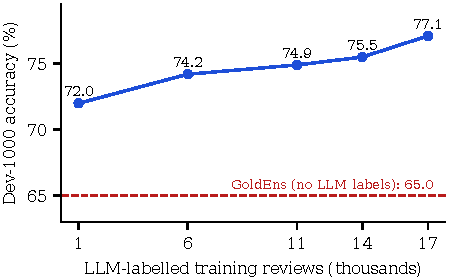
\includegraphics[width=0.85\columnwidth]{fig3_al_scaling.pdf}
\caption{Three-class accuracy on the ood1000 development set versus
AL pool size for the SFT$+$v3 mixture (DeepSeek/hybrid teachers;
1K $=$ gold$+$al1000). The curve is monotone but every point is a
best-of-$N$ development estimate (\S\ref{sec:res-provenance}).}
\label{fig:al-scaling}
\end{figure}

\subsection{Generalization on Human-Labeled Reviews: human400}
\label{sec:res-human400}

human400 is the only evaluation set in this paper with \emph{zero
known identifier overlap} with any training pool and fully human
labels: 400 corpus reviews, length-stratified (160/120/80/40),
identifier-excluded and blind-labelled by a single author
(\S\ref{sec:data}; Appendices~\ref{app:annotation}, \ref{app:human400}).
Labels: 156~positive / 179~neutral / 65~negative; single-annotator,
so no human--human IAA is available, and the stratified sample is a
benchmark, not a population estimate. A text-level overlap audit
(exact, normalized, near-duplicate) found zero exact or
near-duplicate overlap with the pools of evaluated systems and only
two ultra-short normalized matches in corpus pseudo-label pools
(Appendix~\ref{app:human400}).

On it, deployed v3 reaches 55.8\% three-class accuracy (macro-F1
55.4) and 76.5\% binary accuracy on the 221 non-neutral rows---far
below its dev-set estimates and exactly matched by the star-rating
lookup of \S\ref{sec:res-rating} (223/400 $=$ 55.75\%; per-rating,
only 62.7\% of 5-star and 50.7\% of 4-star reviews are labelled
positive by the annotator).

The frozen-weight al17k mixture reaches \textbf{64.8\%} three-class
accuracy (macro-F1 63.5), $+9.0$pp over both v3 and the star lookup.
The gain is real but its significance is concentrated: raw McNemar
tests give $p{=}1.3{\times}10^{-3}$ versus v3 and $7.4{\times}10^{-3}$
versus the star lookup; under Holm correction over the 16 pairwise
human400 comparisons (Appendix~\ref{app:human400}) only the
mix-vs-v3 result survives (adjusted $p{=}0.021$; mix-vs-star
adjusted $p{=}0.104$). This \emph{reverses} the teacher-alignment
worry: on identifier-disjoint human labels the AL gains are genuine
generalization over the deployed system, though the margin over a
rating baseline is nominally, not family-wise, significant.
Per-class, the gain is a neutral-class repair: neutral F1
rises 55.9$\to$68.0 (recall 50.3$\to$73.7) while negative recall
drops 81.5$\to$66.2 in exchange for much higher negative precision
(35.3$\to$54.4); full per-class precision/recall/F1 for all five
systems is in Appendix~\ref{app:human400}
(Table~\ref{tab:human400-perclass}). Caveats: accuracy on
annotator-flagged \emph{mixed} reviews drops below v3 (40.0\% vs.\
53.3\%, $n{=}30$); Qwen3-4B zero-shot reaches 61.5\%/59.0, below the
mixture (raw McNemar $p{=}0.26$).

Binary ($n{=}221$): v3 reaches 76.5\%, below the rating rule (83.7\%),
which the frozen mixture \emph{matches exactly} (83.7\%) while
predicting a more balanced class distribution and a higher macro-F1
(81.3 vs.\ 77.9). The two make identical numbers of errors in
opposite directions (28/28 symmetric discordance, $p{=}1.0$), so the
binary gain over the rating rule is class balance, not accuracy;
versus v3 the raw McNemar $p{=}0.020$ does not survive Holm correction
(adjusted $p{=}0.234$; Appendix~\ref{app:human400}).

\subsection{Annotation Provenance and Evaluation Sensitivity}
\label{sec:res-provenance}

Every number in this paper means something different depending on
where its labels came from and how the model was selected: leakage-
channel ablations on the gold OOF estimates, the development-set
status and provenance of ood1000, and row-level train/test
contamination.

\paragraph{Gold-OOF leakage decomposition.}
Table~\ref{tab:main-results} contrasts our previously reported
(uncorrected) headline with the leakage-reduced $\alpha{=}1.0$ rerun.
The three-class deployed 89.5\%/85.9\% decomposes cleanly: Leak~B
(second-order teacher targets) accounts for $+5.5$pp accuracy
($89.5\to84.0$ with the corpus channel kept), and the transitive
corpus channel (Leak~A) contributes a further $+0.7$pp that vanishes
when removed ($84.0\to83.3$), leaving a leakage-reduced OOF range of
\textbf{83.3--84.0\% accuracy / 76.3--77.8 macro-F1} (the deduplicated
rerun reported with the ablations gives 82.6--83.1\%). The binary
pipeline has no corpus channel, so its entire inflation ($+3.0$pp) is
Leak~B, leaving \textbf{92.9\%/92.4\%} (91.5\%/90.8 deduplicated).
These are leakage-channel ablation estimates, not a fully nested,
selection-independent final-system score (single seed, frozen weights
tuned on gold-600, $\alpha{=}1.0$ not re-tuned, residual
duplicate-text channel; \S\ref{sec:res-ablations}). Our earlier
headline claims were inflated; the honest numbers are the
contribution.

\begin{table}[t]
\centering
\scriptsize
\begin{tabular*}{\columnwidth}{@{\extracolsep{\fill}}lp{3.5cm}cc@{}}
\toprule
Task & Pipeline variant & Acc & Macro-F1 \\
\midrule
\multirow{4}{*}{3-class}
 & deployed, uncorrected ($\alpha{=}0.5$) & 89.5 & 85.9 \\
 & $\alpha{=}1.0$, corpus kept & 84.0 & 77.8 \\
 & $\alpha{=}1.0$, corpus removed & 83.3 & 76.3 \\
 & $\alpha{=}0.5$, corpus removed & 87.5 & 81.3 \\
\midrule
\multirow{2}{*}{binary}
 & deployed, uncorrected ($\alpha{=}0.5$) & 95.9 & 95.6 \\
 & $\alpha{=}1.0$ (no corpus channel) & 92.9 & 92.4 \\
\bottomrule
\end{tabular*}
\caption{Gold-600 out-of-fold results (\%). ``Uncorrected'' rows are the
previously reported deployed scores; $\alpha{=}1.0$ rows remove second-order
teacher leakage (Leak~B). The corpus-channel toggle bounds Leak~A.
Leak~B $\approx{+}5.5$pp (3-class) / ${+}3.0$pp (binary); Leak~A
$\approx{+}0.7$pp.}
\label{tab:main-results}
\end{table}

\paragraph{ood1000 is a development set.} Every Stage-2 decision was
read off ood1000 accuracy: AL scale (1K$\to$17K), teacher choice
(DeepSeek/Qwen/hybrid), per-task epochs, seed count and subset, and
fusion weights via cross-validation on ood1000 itself---26 mixture
configurations and $\approx$73 SFT runs in total. OOD claims are only
as honest as the selection protocol behind them \citep{baran2023ood};
we therefore report ood1000 numbers as \emph{development estimates}
with an estimated best-of-$N$ optimism of $+0.3$--$1.0$pp (3-class)
and $+0.2$--$0.7$pp (binary), and McNemar tests on this set are
anti-conservative because it was reused for selection.

\paragraph{Row-level contamination.} Our cid audit
(Appendix~\ref{app:audit}) shows evaluation texts entered corpus
training sets: 68.7\% of ood1000, 70.2\% of fresh500, and 74.8\% of
lab500 rows share a corpus ID with at least one corpus-trained model,
plus 220/107 near-duplicate rows on ood/fresh; the deployed neutral
detector trained on 13.0\%/13.2\% of ood1000/fresh500. AL/SFT pools
have \emph{zero} cid overlap, so SFT-mix gains cannot be explained by
row memorization, but every corpus-channel number carries bounded
exposure.

\paragraph{Label provenance splits the benchmark.}
Table~\ref{tab:ood-results} splits ood1000 by label provenance. Every
system drops 20--32pp on the 200 human-adjudicated rows---though this
gap confounds label source with item difficulty, since the adjudicated
rows are exactly the disagreement-enriched, harder items. On this
subset the ranking changes: DeepSeek-V4.1-Flash zero-shot (59.5\%,
$n{=}195$ parseable) \emph{exceeds} our best local mixture (56.0\%),
while v3 falls to 46.5\%. The two LLM passes agree on only 29.8\% of
the 47 adjudicated rows ($\kappa{=}{-}0.18$) versus 100\% on consensus
rows by construction, indicating consensus labels encode a single
model's conventions \citep{schroeder2025humanloop,moller2024parrot}
---part of the mixture's consensus-subset lead is label-convention
alignment, not broad generalization. Binary is more robust: the best
mix loses only 8.4pp across provenance (93.7$\to$85.3) versus 26.4pp
three-class.

\paragraph{fresh500 is a partially exposed replication.}
On \textbf{fresh500}---zero text overlap with gold/AL pools but
$\sim$70\% comment-ID overlap with corpus-derived training and
DeepSeek-Flash labels from the same teacher family as $\approx$16K AL
labels---the fixed al17k recipe replicates at 77.0\%/93.7\% versus
v3's 58.8\%/86.3\%, but it measures agreement with teacher
conventions as much as generalization, and only the top-2 ood1000
configurations were evaluated on it.

\begin{table}[t]
\centering\scriptsize
\setlength{\tabcolsep}{2.5pt}
\begin{tabular}{llcccc}
\toprule
Eval rows & $n$ & v3 & al17kds mix & DS-Flash & Qwen3-4B \\
\midrule
ood1000, all (dev) & 1000 & 65.0 & 77.1 & 82.0 & 70.6 \\
\quad LLM-consensus & 800 & 69.6 & 82.4 & 87.5 & 75.1 \\
\quad human-adjudicated & 200 & 46.5 & 56.0 & 59.5 & 52.5 \\
\midrule
fresh500 (DS labels) & 500 & 58.8 & 77.0 & --- & --- \\
\midrule
human400 (blind human) & 400 & 55.8 & 64.8 & --- & 61.5 \\
\bottomrule
\end{tabular}
\caption{3-class accuracy (\%) by evaluation set and label provenance.
ood1000 is a development/selection set; its 200 adjudicated rows were
labelled with student predictions visible, and the consensus-vs-
adjudicated gap confounds label source with item difficulty
(\S\ref{sec:res-provenance}). DS-Flash is scored on its parseable rows
only: $n{=}992/797/195$ of the 1000/800/200 rows above; all other
columns use every row. human400 labels are single-author blind
annotations on an identifier-disjoint, length-stratified sample; mix
uses frozen ood1000-selected weights (\S\ref{sec:res-human400}).}
\label{tab:ood-results}
\end{table}

\subsection{Model Ablations and Error Analysis}
\label{sec:res-ablations}

\paragraph{Duplicate-text leakage.} A further channel affects even the
$\alpha{=}1.0$ estimates: gold-600 has 600 rows but only 592 unique
texts---8 exact-duplicate pairs (Appendix~\ref{app:audit})---and every
OOF script uses stratified $k$-fold without group constraints, so
duplicates can cross folds (expected $\approx$6--7 of 8 pairs),
violating per-fold isolation; we estimate the inflation at $\sim$1--2pp,
concentrated in neutral/negative classes. Retraining the full pipeline
on the 592 unique texts with dedup-aligned teachers moves the
$\alpha{=}1.0$ estimates to \textbf{82.6--83.1\%} three-class /
74.8--75.9 macro-F1 and \textbf{91.5\%} / 90.8 binary (from 83.3--84.0
/ 76.3--77.8 and 92.9 / 92.4 on the 600 rows); the $\alpha{=}0.5$
variant drops more (86.5\% vs.\ 89.5\%). These deduplicated
leakage-reduced OOF estimates are the in-domain numbers we stand behind.

\paragraph{Diagnostics and negative results.}
Appendix~\ref{app:ablations} collects the statistical diagnostics:
adjacent AL scales are within noise (al17kds\_avg5 vs.\
al14kds\_avg: $+1.6$pp, McNemar $p{=}0.064$); the v2$\to$v3
neutral-correction gain is positive but non-significant
($\Delta$macro-F1 $+1.6$pp; bootstrap 95\% CI $[-0.4,+3.8]$pp;
McNemar $p{=}0.65$); the OOD drop is \emph{not} a short-text artifact
(neutral recall collapses 51.1$\to$33.3\% across ood1000 length
buckets); and IAA is $\kappa{=}0.568$ against a \emph{blended}
human/LLM reference only. Over twenty variants were rejected
(Appendix~\ref{app:negative}); headline selection thus operated on
ood1000, and a fold-isolated corpus detector, re-tuned fusion weights,
and a second human400 annotator would further change our conclusions.
